%!TEX root = ../dokumentation.tex

\chapter{Theoretische Hintergründe}\label{theoretische_hintergründe}
\nocite{*}

In diesem Kapitel werden die theoretischen Hintergründe zur Spieletheorie im Generellen und vor Allem der Entwicklung von Spiele-Spielenden-Computern eingegangen. Dies wird im Verlauf der Kapitel stets auf das Spiel Schach spezialisiert, da sich der Schwerpunkt dieser Arbeit auf dieses Spiel fokussiert. 
Zunächst werden die klassischen Spieletypen nach der Spieletheorie betrachtet und Schach in diese Kategorien eingeordnet. Darauf folgend wird als Einführung zu Spiele-\acs{KI}s (\acl{KI}) die Geschichte der Entwicklung dieser betrachtet, um Zusammenhänge mit technischen und mathematischen Fortschritten besser zum Verständnis zu bringen.

Anschließend wird speziell auf Algorithmen zur Entwicklung einer Spiele-KI von sequenziellen Nullsummenspielen wie Schach eingegangen. Dabei wird zuerst der grundlegende ``Minimax-Algorithmus'' betrachtet und zudem auf die Optimierung dieses durch ``Alpa-Beta Pruning'' eingegangen. Darauffolgend werden zudem die Problematiken der Anwendung dieser auf komplexe Spiele beschrieben und mögliche Lösungen vorgeschlagen. 

Abschließend für dieses Kapitel werden durch genannte Problematiken nötig werdende Evaluierungsfunktionen der einzelnen Spielzustände im Spiel Schach genannt und beschrieben, womit die theoretische Grundlagenschaffung für das Entwickeln einer Schach-KI abgeschlossen ist.

\section{Einordnung der Spieltypen für Schach} \label{game_types}

In der klassischen Spieletheorie werden Spiele anhand von fünf Kategorien unterschieden und eingeordnet. Diese fünf Kategorien sind
\begin{itemize}
\item Symmetrische / Asymmetrische Spiele
\item Vollständige / Unvollständige Informationslage
\item Kooperative / Nicht-kooperative Spiele
\item Simultane / Sequentielle Spiele
\item Nullsummenspiele / Nicht-Nullsummenspiel \cite{Rodriguez}
\end{itemize} 

Diese werden nun alle einzeln beschrieben sowie der Unterschied erläutert. Außerdem wird das Spiel Schach jeweils einer der Spieltypen zugeordnet.

Im ersten Schritt wird zwischen symmetrischen und asymmetrischen Spielen unterschieden. Bei symmetrischen Spielen hat jeder Spieler dieselben Ziele, um das Spiel zu gewinnen. Der Sieg ist dabei abhängig von den gewählten Strategien. Bei asymmetrischen Spielen dagegen verfolgen die teilnehmenden Parteien unterschiedliche Ziele. \cite{Rodriguez} Ein klassisches Beispiel ist dabei das Spiel des Jägers und des Gejagten - während der Jäger versucht den Gejagten zu fangen, versucht der Gejagte zu entkommen. Unter Umständen wird auch der Erfolg im Nachhinein anhand verschiedener Kriterien evaluiert, so dass unter Umständen beide Seiten für sich einen Sieg erringen können.

Schach stellt dabei ein klassisches Beispiel eines symmetrischen Spiels dar. Beide Seiten versuchen jeweils den gegnerischen König Schachmatt zu setzen, ohne dabei selbst zuvor Schachmatt gesetzt zu werden.

Vollständige und unvollständige Informationslagen in Spielen kategorisieren Spiele nach dem Wissen, den der Spieler über das Spiel hat. Vollständige Informationslage bedeutet, dass der Spieler über alle getätigten Züge und Spielzustände informiert ist und nicht aus Unwissenheit heraus agieren muss. Bei unvollständiger Informationslage ist das Gegenteil der Fall. \cite{Rodriguez} Bei vielen Kartenspielen beispielsweise, wie Poker oder Black Jack, hat ein Spieler keine Informationen über die Karten in der Hand der anderen Spieler. Dies ist dann als unvollständige Informationslage zu bezeichnen.

Im Spiel Schach jedoch sind die Figuren und dessen Positionen beider Spieler für alle Seiten offengelegt und einsehbar. Dadurch können sich beide Spieler ein Gesamtbild über die Situation machen, ohne dass ein Mangel an Information herrscht.

Bei kooperativen Spielen handelt es sich um Spiele, in denen mehrere Spieler zusammen an einem Ziel arbeiten können oder gar müssen, um ihr Ergebnis zu verbessern. Dies kann in Bündnissen münden, die mehrere Spieler zusammen eingehen, um an einem Ziel zu arbeiten, dass alle gemeinsam erreichen können. \cite{Rodriguez} Ein Beispiel dafür sind ist das Spiel Scotland Yard. Dabei müssen verschiedene Spieler zusammen arbeiten, um einen Spieler, der die Rolle des Mister X übernimmt, ausfindig zu machen. Dazu müssen sie Hinweise des Aufenthaltortes nutzen und den Gegenspieler dann gemeinsam versuchen zu umstellen, so dass dieser nicht mehr fliehen kann. Es ist also eine direkte Zusammenarbeit mehrerer Spieler nötig, um das Spiel gewinnen zu können. \cite{Ravensburg2000} In Nicht-kooperativen Spielen dagegen ist es verboten oder nicht zielführend Allianzen zu formen, da kein gemeinsamer Sieg errungen werden kann. \cite{Rodriguez}

%https://www.ravensburger.com/spielanleitungen/ecm/Spielanleitungen/Scotland_Yard_W_And_B_GB.pdf

Schach stellt dabei ein Nicht-kooperatives Spiel dar, da die Spieler nicht miteinander, sondern nur gegeneinander antreten können.

Simultane Spiele sind Spiele, bei denen alle Spieler gleichzeitig Aktionen unternehmen können. Ein Beispiel stellt dabei ein Kampf dar, in der beide Seiten sich gleichzeitig bewegen können und in Echtzeit auf die Bewegungen des Gegners reagieren müssen. Bei sequenziellen Spielen dagegen wechseln sich alle Seiten mit ihren Zügen ab. Dies bedeutet auch, dass die Spieler über die vorangegangenen Züge ihrer Gegner Bescheid wissen. \cite{Rodriguez}

Wie die meisten Brettspiele stellt Schach dabei ein sequentielles Spiel dar. Die Spieler wechseln sich mit ihren Zügen ab und wissen über die durch den Gegner bewegten Figuren Bescheid.

Als letzte Unterscheidung gelten Nullsummenspiele und Nicht-Nullsummenspiele. Bei Nullsummenspielen ist Gewinn für den einen Spieler immer einhergehend mit einem gleichzeitigen Verlust für einen anderen Spieler. Dies bedeutet, dass Werte für Gewinn und Verluste für alle Spieler zusammen gerechnet immer auf den Wert Null hinauslaufen. Bei Nicht-Nullsummenspielen ist dies nicht der Fall. Dabei können von einer Aktion eines Akteurs mehrere Akteure gleichzeitig profitieren, ohne dass andere darunter leiden.\cite{Rodriguez} Ein Beispiel dafür ist das Gefangenendilemma. Dabei können zwei Gefangene jeweils die Entscheidung treffen, ob sie ihr Verbrechen gestehen oder Schweigen. Von ihrem Handeln sowie dem Handeln der anderen Partei hängt die Länge ihrer Strafe ab. \cite{Tweedale1993} Diese ist folgender Tabelle zu entnehmen:

\begin{tabular}{l c c}
& \textbf{B schweigt} & \textbf{B gesteht} \\
\textbf{A schweigt} & A: 2 Jahre; B: 2 Jahre & A: 6 Jahre; B: 1 Jahr \\
\textbf{A gesteht} & A: 1 Jahr; B: 6 Jahre & A: 4 Jahre; B: 4 Jahre
\end{tabular}

%Tweedale, G. (1993). William Poundstone, Prisoner's Dilemma: John von Neumann, Game Theory, and the Puzzle of the Bomb. Oxford: Oxford University Press, 1992. Pp. xi 290. ISBN 0-19-286162-X. £7.99 (paperback edition). The British Journal for the History of Science, 26(3), 375-376. doi:10.1017/S0007087400031332

Dies ist als klassisches Nicht-Nullsummenspiel bekannt, da beide Seiten je nach Reaktion zusammengerechnet minimal 4 Jahre und maximal 8 Jahre Strafe bekommen. Somit ist das Gesamtergebnis nicht stets das gleiche und beide Seiten können von gegenseitigem Schweigen profitieren.

Anders ist dies bei Schach. Schach ist als Nullsummenspiel zu betrachten, da am Ende des Spiels immer entweder eine Seite gewonnen (+1) und die andere verloren (-1) hat oder beide Seiten ein Unentschieden/Patt erreicht haben (0).

Nachdem nun Schach in die Spieletheorie-Typen eingeordnet ist, wird in folgenden Kapiteln näher auf die Möglichkeiten zur Durchführung des Schach Spiels durch einen Computer eingegangen.

%What Data Scientists Should Know About Game Theory: Types of Games


\section{Geschichte der Spieltheorie}\label{history}

Die Geschichte der Spieltheorie im Computerumfeld beginnt mit Claude Shannon im Jahre 1949, als dieser seine Gedanken zur möglichen Realisierung eines Schach spielenden Computers veröffentlicht. Dabei begründet er zunächst seine Auswahl auf das Spiel Schach für sein langfristiges Ziel eines spielenden Computers und legt dann das Ziel an sich fest.

\begin{quote}
“The chess machine is an ideal one to start with, since: (1) the problem is sharply defined both in allowed operations (the moves) and in the ultimate goal (checkmate); (2) it is neither so simple as to be trivial nor too difficult for satisfactory solution; (3) chess is generally considered to require ‘thinking’ for skillful play; a solution of this problem will force us either to admit the possibility of a mechanized thinking or to further restrict our concept of ‘thinking’; (4) the discrete structure of chess fits well into the digital nature of modern computers. … It is clear then that the problem is not that of designing a machine to play perfect chess (which is quite impractical) nor one which merely plays legal chess (which is trivial). We would like to play a skillful game, perhaps comparable to that of a good human player.” \cite{Shannon1950}
\end{quote} 

Der vorgeschlagene Ansatz zum Evaluieren der Züge stellt dabei ein Algorithmus dar, der heute unter ``Minimax-Algorithmus'' bekannt ist. Dieser Ansatz wird in Kapitel \ref{minimax} erklärt.

%http://www.andreykurenkov.com/writing/ai/a-brief-history-of-game-ai/

Anwendung fand dies erstmals im Jahre 1956, als ein Team von Mathematikern und Forschern um Arthur Samuel ein Programm entwickelten, das in der Lage war ``Dame'' zu spielen. Dies war das erste Mal, das ein Computer in der Lage war in einem strategischen Spiel gegen einen Menschen anzutreten. Im Rahmen dieses Projekts ist auch der Begriff ``Artificial Intelligence'' oder zu deutsch ``Künstliche Intelligenz'' entstanden. \cite{Kurenkov2019}

Dabei wird vom aktuellen Zustand aus einige Züge vorausgeschaut und bewertet, welcher Zug unter der Annahme, dass auch der Gegner den jeweils besten Zug machen wird, der aussichtsreichste ist. Zur Berechnung wird ein Minimax Baum ausgehend von der aktuellen Spielsituation aus erstellt.

%image?

Auch wurden hier erste Machine-learning Algorithmen verwendet, die dem Computer innerhalb kürzester Zeit das Spiel so gut beibringen, dass dieser dazu in der Lage ist menschliche Spieler zu schlagen. Samuel verwendete dazu zwei Methoden - Einerseits  das "Auswendiglernen", das die Werte von bestimmten Spielzuständen, die bereits evaluiert wurden, abspeichert, so dass die Berechnung kein weiteres Mal durchgeführt werden muss. Zum anderen ``learning-by-generalization'', das die Parameter der Evaluierungsfunktionen basierend auf vorherigen Spielen anpasst. Dies geschah mit dem Ziel, den Unterschied zwischen dem berechneten Evaluierungswert des Zustands und dem tatsächlichen, auf den Ausgang des jeweiligen Spiels basierenden Werts zu minimieren. \cite{Samuel1959}

%https://www.cs.virginia.edu/~evans/greatworks/samuel1959.pdf

Nur ein Jahr später fand die Theorie von Claude Shannon auch erstmals direkt im Spiel Schach Anwendung. Ein Team um den Mathematiker Alex Bernstein entwickelte eine voll funktionale Schach- KI, ebenfalls basierend auf den Minimax Algorithmen. \cite{Kurenkov2019} Die Problematik beim Schach, im Vergleich zu anderen Spielen, ist die enorme Anzahl an verschiedenen Zügen und Spielzuständen, die eine Evaluierung jedes einzelnen, selbst bei heutiger Rechenkapazität, unmöglich macht. Dies ist genauer in Kapitel \ref{depth_limit} beschrieben. 

Auf Grund dieser Komplexität des Schach Spiels, sowie der begrenzten Rechenkapazitäten der damaligen Computer, wurde dies auf eine Tiefe von vier begrenzt. Dies bedeutet, dass der Computer lediglich vier Züge vorausschaut. Zusätzlich schaut der Computer lediglich sieben verschiedene Optionen pro Zug an. Die Auswahl dieser sieben Optionen geschah mittels simpler heuristischer Berechnungen, die versuchten im Vorab die sieben aussichtsreichsten Optionen zu wählen. \cite{Bernstein1958}

%Minimax Tree image?

Diese Limitationen jedoch ermöglichten lediglich ein relativ simples, wenn auch passables Schachspiel.

%https://d1yx3ys82bpsa0.cloudfront.net/chess/computer-v-chessplayer.bernstein-roberts.scientific-american.june-1958.062303059.pdf

Um die Zahl der zu evaluierenden Züge zu reduzieren, wurde im Jahr 1958 von Allen Newell und Herbert Simon eine Modifizierung des Minimax Ansatzes veröffentlicht - genannt ``alpha beta pruning''. Diese Modifizierung verhindert das Evaluieren von Zügen, die eindeutig schlechter sind. Dieser Ansatz wird genauer in Kapitel \ref{alpha_beta} beschrieben. \cite{Newell2010}

%Allen Newell, Cliff Shaw, Herbert Simon (1958). Chess Playing Programs and the Problem of Complexity. IBM Journal of Research and Development, Vol. 4, No. 2, pp. 320-335. Reprinted (1963) in Computers and Thought (eds. Edward Feigenbaum and Julian Feldman), pp. 39-70. McGraw-Hill, New York, N.Y. pdf

Diese neue Vorgehensweise kann einiges an Rechenkapazitäten sparen und soll so zum ersten Mal einen menschlichen Spieler geschlagen haben, der das Spiel allerdings erst kurz zuvor erlernt hatte. \cite{Kurenkov2019}

Durch Verbesserung der Algorithmen und erweiterten Rechenkapazitäten durch immer bessere und performantere Computer, teilweise extra optimiert auf das Schach Spiel, konnten Stück für Stück neue Erfolge erzielt werden. 1962 konnte eine KI von Arthur Samuel erstmals einen renommierten Spieler, Robert Nealy, schlagen. \cite{Kurenkov2019}

1994 konnten die besten Dame Spieler der Welt eine KI namens ``CHINOOK'' nur noch ein Unentschieden abverlangen. \cite{Schaeffer1996} Bereits 1988 gelang einem Programm namens ``Deep Thought'' von Feng-hsiung Hsu, später von IBM weiterentwickelt unter dem Namen ``Deep Blue'' bekannt, ähnliches im Schach Spiel und schlug den Schach-Großmeister Bent Larsen. Im Jahre 1997 schlug die weiterwntickelte Version "Deep Blue" Schachweltmeister Kasparov.\cite{Kurenkov2019}

Beide Programme basierten dabei auf drei wesentlichen Punkten: Eine Datenbank von Eröffnungszügen entnommen von professionellen Spielern, alpha-beta Suchbäume mit einer Menge an Evaluierungsfunktionen sowie einer Endspiel Datenbank sobald nur noch eine geringe Anzahl an Spielfiguren existiert. \cite{Kurenkov2019}

%http://www.andreykurenkov.com/writing/ai/a-brief-history-of-game-ai-part-2/

Diese Programme benötigten speziell optimierte Computer, die auf die nötigen Berechnungen für die jeweiligen Spiele ausgelegt waren. Anders handhabt es das Programm ``Stockfish'' aus dem Jahre 2008. Dies ist auf jedem Computer ausführbar und dennoch für einen Menschen nicht schlagbar.

Lange war Stockfish unbesiegt, dies änderte sich jedoch im Jahr 2017 als AlphaZero mit 64:36 gegen Stockfish gewann. AlphaZero ist dabei ein verallgemeinerter Ansatz von AlphaGo Zero. Dies wiederum ist eine Aktualisierung von AlphaGo, das im Jahr 2017 den Weltmeister in Go schlug. Dabei verwendet AlphaGo neuronale Netzwerke und verwendet Methoden des ``supervised learning'' und ``reinforcment learning'', um sich selbstständig weiter zu entwickeln. \cite{Fischer}

%L. Fischer Künstliche Intelligenz schlägt...

An diesem Punkt endet die Entwicklung von immer besser werdenden KIs jedoch nicht. Besonders durch den Fortschritt im Bereich der neuronalen Netze und speziell im ``Deep Learning'' Bereich werden immer komplexere Spiele durch den Computer beherrscht, immer öfter auch besser als vom Menschen. Ein Beispiel stellt dabei Alpha Star dar, das im Jahre 2019 eines der besten Teams im Echtzeit-Strategiespiel ``Starcraft 2'' geschlagen hat. Diese Entwicklung wird sich wohl auch in den kommenden Jahren fortsetzen, auch außerhalb der Spiele Szene, weshalb KI in unserer Gesellschaft immer mehr an Bedeutung gewinnt. \cite{OriolVinyalsIgorBabuschkinJunyoungChungMichaelMathieuMaxJaderbergWojtekCzarneckiAndrewDudzikAjaHuangPetkoGeorgievRichardPowellTimoEwaldsDanHorganManuelKroissIvoDanihelkaJohnAgapiouJunhyukOhValentinDalibard}

%AlphaStar: Mastering...

\section{Minimax-Algorithmus}\label{minimax}

Der Minimax Algorithmus basiert auf dem ``Minimax-Theorem'' von John von Neumann.

Das Theorem lautet für zwei Personen Spiele:

Dabei wird das Spiel von Spieler A gestartet, der somit zuerst einen Zug wählt. Die Annahme dabei ist, dass Spieler A davon ausgeht, dass Spieler B stets den für ihn besten Zug spielen wird. Das bedeutet, dass Spieler A den Zug wählt, bei der unter dieser Annahme dennoch das beste Endergebnis zu erreichen ist. Hat Spieler A also eine Menge $S$ an Zügen zur Auswahl, werden alle Szenarien von jedem Zug $s \in S$ evaluiert. Die Bewertungsfunktion dieser Züge definieren wir mit

\begin{equation}
\mathtt{utility}: S \times \mathtt{Player} \rightarrow \mathbb{R}
\end{equation}

wobei $S$ für die Menge der Züge steht und $\mathtt{Player}$ für die Menge der Spieler. Aus der Angabe eines Zuges und eines Spielers aus den jeweiligen Mengen ergibt sich eine rationale Zahl, die als Bewertung des Zuges zu betrachten ist. Dabei gilt: Umso höher die Zahl, desto besser der Zug für den angegebenen Spieler.

Dann wird das Minimum aller Bewertungen der Endzustände für jeden Zug $s \in S$ gewählt. Diesen Zug nennen wir $\min (S)$ und dessen Bewertung somit $\mathtt{utility}(\min (s, p)))$, wobei gilt $s \in S$ und $p \in \mathtt{Player}$. Nun wird der Zug $s_{best} \in S$ gewählt, so dass gilt:

\begin{equation}
\forall s \in S : (s \neq s_{best} \rightarrow \mathtt{utility}(\min(s, p)) \leq \mathtt{utility}(\min(s_{best})))
\end{equation}

Anders ausgedrückt - existiert also eine Menge X von Strategien von Spieler A und eine auf X folgende Menge Y von möglichen Strategien von Spieler B, so lautet die Optimierungsregel für Spieler A

\begin{equation}
\max\limits_X[\min\limits_Yu(X,Y)]
\end{equation}

Umgekehrt versucht Spieler B das für Spieler A ungünstigste Ergebnis zu wählen und wählt daher die Strategie, die das Minimum der für Spieler A jeweils nach dem Zug noch bestmöglichen Ergebnisse versprechen. Somit lautet die Optimierungsregel für Spieler B

\begin{equation}
\min\limits_Y[\max\limits_Xu(X,Y)]
\end{equation}

%Strategische Spiele

Dadurch kann Spieler B den Ertrag des Spielers A auf diesen Wert begrenzen. Es gilt also

\begin{equation}
\max\limits_X[\min\limits_Yu(X,Y)] \leq \min\limits_Y[\max\limits_Xu(X,Y)] \cite{Dresher1961}
\end{equation}

Das Theorem geht dabei davon aus, dass es also einen Sattelpunkt $v$ geben muss, bei dem sich die beiden Optimierungen für Spieler A und B einpendeln. Dieser Sattelpunkt lautet

\begin{equation}
\max\limits_X[\min\limits_Yu(X,Y)] = \min\limits_Y[\max\limits_Xu(X,Y)] = v \cite{Dresher1961}
\end{equation}

Diese Strategie basiert auf puren Berechnungen und ist für einen Computer somit leicht durchführbar. Dafür verlangt es folgende Informationen \cite{Stroetmann2018}:

\begin{itemize}
\item \textbf{$\mathtt{States}$}: Alle möglichen Zustände des Spiels
\item \textbf{$s_0$}: Anfangszustand des zu betrachtenden Spiels
\item \textbf{$\mathtt{Player}(s)$}: Gibt den Spieler zurück, der in gegebenem Zustand am Zug ist
\item \textbf{$\mathtt{actions}(s)$}: Eine Liste aller möglichen Züge ausgehend von Zustand s
\item \textbf{$\mathtt{result_states}(s,a)$}: Der von Zustand s über Zug a erreichbare Zustand
\item \textbf{$\mathtt{terminal_test}(s)$}: Prüft einen Zustand darauf, ob dieser das Ende des Spiels bedeutet. Diese wird definiert als

\begin{equation}
\mathtt{terminal_test} : States \rightarrow \mathbb{B}
\end{equation}

wobei $\mathbb{B}$ einem Boolean-Wert, sprich wahr oder falsch, entspricht.

Mittels dieser Funktion kann eine Menge $terminal\_states$ als Menge aller Endzustände gebildet werden:

\begin{equation}
\mathtt{terminal_states} := \{s \in S | \mathtt{terminal_test}(s)\}
\end{equation}

\item \textbf{$utility(s, p)$}: Bewertet einen Zustand, indem sie diesem einen numerischen Wert zuweist. Diese Funktion ist definiert durch

\begin{equation}
\mathtt{utility} : \mathtt{terminal_states} \times \mathtt{Player} \rightarrow \mathbb{R}
\end{equation}

wobei diese den Zustand aus Sicht des gegebenen Spielers bewertet. Umso höher das Resultat dieser Berechnung also, desto besser das Ergebnis für Spieler P.
\end{itemize}

Um die erreichbaren Zustände zu erhalten, benötigt es einen Algorithmus, der anhand der Spielregeln und eines Ausgangszustands $s_0$ und einer Liste aller Züge von s $\mathtt{actions}(s)$ alle erreichbaren Zustände $result_states$ berechnet. Von jedem Zustand $s \in \mathtt{result_states}$ wird dann wiederum jeder mögliche erreichbare Zustand berechnet. Diese Schleife wird fortgeführt, bis die berechneten Zustände den Status einen Endzustand erreichen. Der Fall ist dies, wenn $\mathtt{terminal_test}(s) = \mathtt{True}$ ergibt und somit von diesem Zustand aus keine Änderungen mehr möglich sind.

Entscheidend für die Wahl eines Zuges ist dann die Bewertung jedes einzelnen Zustandes. Dies ist solange umsetzbar, wie der Computer ohne Probleme alle möglichen Zustände berechnen und evaluieren kann. Um dies an einem Beispiel zu zeigen - Beim Spiel ``Tic Tac Toe'', bei dem in einem 3x3 Feld zwei Spieler gegeneinander antreten mit dem Ziel drei aneinander angrenzende (vertikal, horizontal oder diagonal) Felder mit ihrer Figur zu belegen, gibt es insgesamt 255.168 verschiedene Spielverläufe. \cite{Kaplan2017} Diese sind von heutigen Computern in akzeptabler Zeit berechen- und auswertbar.

%https://books.google.de/books?id=mUIzDwAAQBAJ&pg=PT18&lpg=PT18&dq=tic+tac+toe+m%C3%B6gliche+255+168&source=bl&ots=CcuZA068gP&sig=ACfU3U0XQ053sl4-BcVsL-hPnm76l1ZHyg&hl=de&sa=X&ved=2ahUKEwiL_snW6oLhAhXBIVAKHc7tD40Q6AEwAHoECAcQAQ#v=onepage&q=tic%20tac%20toe%20m%C3%B6gliche%20255%20168&f=false

Dazu bildet der Computer einen sogenannten Minimax-Baum und wählt dann den erfolgversprechendsten Zug aus. Nach jedem getätigten Zug werden die erreichbaren Zustände nur noch vom neuen Zustand aus berechnet. Im Spätspiel kann ein solcher Baum bei ``Tic Tac Toe'' beispielsweise aussehen wie in Abbildung \ref{fig:tictactoe_minimax_tree}.

\begin{figure}[h]
\centering
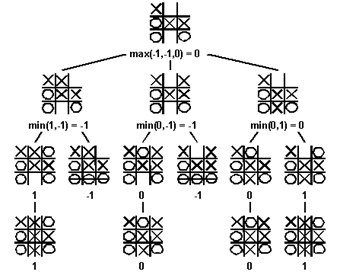
\includegraphics[width=\textwidth/5*3]{images/tictactoe_minimax_tree.png}

\caption{Tic Tac Toe Minimax Baum \cite{Kurenkov2019}}\label{fig:tictactoe_minimax_tree}
\end{figure}
%http://www.andreykurenkov.com/writing/ai/a-brief-history-of-game-ai/

Dabei werden vom Ausgangszustand, der den Zustand des aktuellen Spiels widerspiegelt, aus alle möglichen Folgezustände berechnet. Von diesen werden wiederum alle möglichen Folgezustände berechnet. Dies wird solange fortgeführt, bis alle neu berechneten Zustände Endzustände sind. Dann werden alle Endzustände evaluiert. Eine 1 stellt dabei einen Sieg dar, eine 0 ein Unentschieden und eine -1 eine Niederlage. Da davon ausgegangen wird, dass der gegnerische Spieler stets den besten Zug auswählt, wird jeder Zustand, der noch Folgezustände besitzt, mit dem für ihn schlechtesten Wert aller seiner möglichen Folgezustände bewertet. Der Computer wählt dann den Zustand mit der für ihn besten Bewertung. \cite{Russell2010}
%zu minimax?

In diesem Beispiel wird sich der Computer somit für den dritten Zug von links entscheiden, da bei beiden anderen ein Sieg des Gegenspielers bevorsteht, sollte dieser jeweils die perfekten Züge spielen. Beim dritten Zug kann der Gegner maximal noch ein Unentschieden erreichen.

Diese Strategie gerät jedoch dann an ihre Grenzen, wenn nicht mehr alle möglichen Zustände berechnet werden können. Bei dem Spiel Schach beispielsweise belaufen sich Schätzungen schon nach den ersten 40 Spielzügen auf 10\textsuperscript{115} - 10\textsuperscript{120} verschiedene Spielverläufe. \cite{Bonsdorff1978} Dies ist auch für einen Computer in tolerierbarer Zeit unmöglich berechenbar. Aus diesem Grund muss die Strategie für solch komplexere Spiele abgewandelt werden. Die verschiedenen Ansätze dazu sind in Kapitel \ref{depth_limit} beschrieben.

% Eero Bonsdorff, Karl Fabel, Olavi Riihimaa: Schach und Zahl. 3. Auflage, Rau, Düsseldorf 1978.
%https://de.wikipedia.org/wiki/Schach#cite_note-6

Um diesen Algorithmus in die Praxis umzusetzen, verlangt es drei Funktionen, die jeweils auf den Parameter \textbf{state} angewiesen sind. Dieser Parameter gibt Aufschluss über den aktuellen Zustand des Spiels.

Zusätzlich verlangt der Algorithmus neben der genannten Funktionen $utility$ und $finished$ eine Funktion $min$ sowie eine Funktion $max$, die jeweils mehrere Werte vergleichen und den Minimum bzw. Maximum aller verglichenen Werte zurück geben. Eine beispielhafte Implementierung eines solchen mittels drei verschiedener Funktionen kann in Algorithmus \ref{alg:minimax} gesehen werden.

Die erste Funktion geht dabei jeden möglichen Zug vom gegebenen Ursprungszustand durch und gibt am Ende den Zustand zurück, der den besten Minimum-Wert durch die Evaluierungsfunktion $utility$ erreicht. Dazu gibt die Funktion jeden der erreichbaren Zustände zu der minValue Funktion. Diese gibt entweder den durch die $utility$ Funktion errechneten Wert des Zustands zurück, sollte der Zustand ein Endzustand sein, oder sie gibt das Minimum aller Maxima-Werte der erreichbaren Zustände zurück. Dazu wiederum wird die maxValue Funktion verwendet, die genau das Gegenteil der minValue Funktion macht. Ist der Endzustand erreicht, gibt zwar auch die maxValue Funktion den Wert des Zustands direkt zurück, andernfalls aber gibt sie das Maximum aller Minimum Werte der vom gegebenen Zustand aus erreichbaren Zustände zurück, wozu wiederum auf die minValue Funktion zurückgegriffen wird. Dies ganze wiederholt sich also rekursiv so lange, bis alle neu errechneten Zustände den Wert eines Endzustandes erreicht haben. \cite{Russell2010}

Diesen Endzuständen werden dann Werte zugewiesen, die aufsteigend rekursiv miteinander verglichen und abwechselnd Minimum und Maximum gewählt werden, um dem Minimax-Theorem dahingehend zu folgen. Um das Ganze zu verdeutlichen kann Abbildung \ref{fig:minimax_tree} als Beispiel genommen werden:

\begin{figure}[h]
\centering
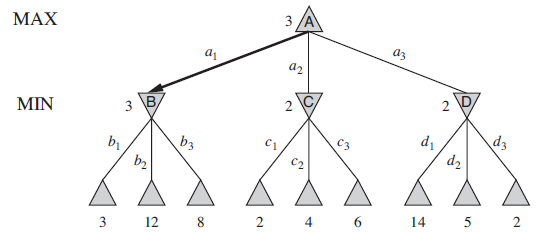
\includegraphics[width=\textwidth/5*4]{images/minimax_algorithm_tree.PNG}

\caption{Minimax Baum \cite{Russell2010}}\label{fig:minimax_tree}
\end{figure}

Dabei hat der gegebene Zustand noch eine erreichbare Tiefe von drei bis alle darauffolgenden Zustände Endzustände sind. Diesen Endzuständen wird dann ein Wert zugewiesen. Nun werden diese Werte auf einer um eins höheren Ebene verglichen. Da es sich hierbei um eine gerade Tiefe (2) handelt, wird hier das Minimum dieser Werte gewählt. Im Knoten B ist dies in unserem Beispiel 3, das 3 der geringste Wert der Endzustände (3, 12 und 8) ist. Im Knoten B sowie D ist jeweils 2 der geringste mögliche Wert. 

Von diesen ausgerechneten Minima wird dann auf Ebene 1 das Maximum berechnet. Das Maximum von 3, 2 und 2 beträgt 3, weshalb der Wert von Knoten B der höchste ist und somit wird der Zug, der zu Zustand B führt, zurückgegeben.

Somit ist es mit dem Minimax-Algorithmus möglich anhand für den Computer möglicher Berechnungen ein Spiel zu evaluieren und den besten Zug zu wählen unter der Annahme, dass der Gegenspieler ebenso handeln wird. Problematisch dabei ist jedoch besonders bei komplexeren Spielen die Dauer der Evaluierung aller Züge. Dies liegt zum einen daran, dass jeder einzelne Zug evaluiert wird und somit bei komplexen Spielen eine enorm hohe Zahl an Zuständen evaluiert werden muss. Zum anderen ist das größte Problem aber wohl, dass es zwangsweise das Spiel bis in die Endzustände berechnen muss, was eine enorm hohe Anzahl an zu evaluierenden Positionen verlangt und somit eine extreme Zeitspanne zum Berechnen mit sich zieht. So ist die Zeitkomplexität bei einem Spiel der Tiefe m und einer Anzahl b an möglichen Zügen gleich $O(b^m)$. \cite[S.169]{Russell2010}
%169


%genaue Zahl?

Das erste Problem, dass jeder einzelne Zug berechnet wird, wird mit dem Ansatz des Alpha Beta Pruning versucht zu minimieren. Dieser Ansatz wird im Kapitel \ref{alpha_beta} erklärt. Das Problem, dass stets bis in die Endzustände gerechnet werden muss, wird in Kapitel \ref{depth_limit} genauer erläutert sowie einige Lösungsansätze dargestellt.

% bessre Überleitung formuliere


%algorithmus in praxis

\section{Alpha-beta pruning}\label{alpha_beta}

Ein Problem bei dem Minimax Algorithmus ist, wie bereits in Kapitel \ref{minimax} angesprochen, die Evaluierung eines jeden möglichen Zuges, obwohl manche Züge eventuell schon im Vorhinein mittels trivialer Berechnungen ausgeschlossen werden können und gar nicht mehr näher betrachtet werden müssten. Auch ein guter Schachspieler geht ja nicht jeden möglichen Zug im Kopf durch, sondern schaut sich nur spezielle Züge bis zu einer gewissen Tiefe an und sobald er erkennt, dass dieser nicht gewinnbringend ist, schließt er diesen direkt aus, ohne ihn weiter zu evaluieren.

Für ein ähnliches Schema gibt es eine erweiternde Technik des Minimax-Algorithmus. Diese nennt sich Alpha-Beta-Pruning. Dabei wird versucht große Teile des Minimax Baums bereits auszuschließen, bei denen auf triviale Weise erkannt werden kann, dass diese die finale Entscheidung nicht beeinflussen würden. 

Durch die Verzweigung von min- und max-Funktionen im Minimax-Baum, können bestimmte Zweige oftmals bereits ausgeschlossen werden, da dieser für das Ergebnis der min-max Verzweigung irrelevant ist. \cite{Russell2010} Um dies an einem Beispiel zu erklären, kann folgende min-max-Verschachtelung dienen:

\begin{equation}
MINIMAX(root) = \max(\min(3,12,8), \min(2,x,y))
\end{equation}

Aus dem ersten min Zweig wird dabei 3 als Gewinner hervorgehen, da es der niedrigste Wert ist. Im zweiten Zweig gibt es mit dem Wert 2 bereits einen potentiellen Gewinner. Auch bei weiterer Evaluierung dieses Zweigs kann höchstens eine noch kleinere Zahl als 2 als Sieger aus dem min Zweig hervorgehen. Da 2 oder eine kleinere Zahl in dem darüberstehenden max-Zweig sich nicht gegen 3 durchsetzen kann, ist die Evaluierung der bisher nicht berechneten Zweige x und y irrelevant, da sie keinen Einfluss auf die Entscheidung haben. Dementsprechend kann diese übersprungen werden. Der Baum sieht dann wie folgt aus

\begin{equation}
\begin{aligned}
MINIMAX(root) &= \max(\min(3,12,8), \min(2,x,y)) &
\\
&= \max(3, \min(2,x,y))&
\\
&= \max(3, z) & \rlap{\footnotesize(where $z = \min(2,x,y) \leq 2$)}
\\
&= 3&
\end{aligned}
\end{equation}

Dabei wird der Term $\min(2,x,y)$ durch z ersetzt, wobei z durch die Eigenschaft $z \leq 2$ definiert wird. Auf Grund dieser Tatsache, kann das Ergebnis des Terms $max(3, z)$ eindeutig auf 3 festgelegt werden.

In Abbildung \ref{fig:alpha_beta_chess} kann dies nochmal anhand eines realen Beispiels von einem Ausschnitt aus einem Schachspiel verdeutlicht werden. 

\begin{figure}[h]
\centering
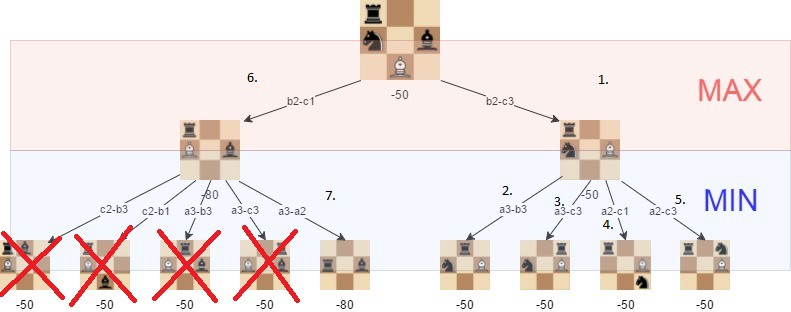
\includegraphics[width=\textwidth]{images/alpha-beta-chess.jpeg}

\caption{Alpha Beta Pruning Beispiel anhand von Schachausschnitt \cite{Hartikka}}\label{fig:alpha_beta_chess}
\end{figure}
%a step by step guide

Gehen wir dabei aus, dass zuerst der rechte Zweig (1.) vollständig evaluiert wurde, wofür zunächst alle Knoten dieses Zweigs (2.-5.) betrachtet wurden. Nach diesen Berechnungen wird Knoten 1 das Minimum aller Zweige von 1 zugewiesen. Dieses beträgt -50. Danach soll der linke Zweig (6.) evaluiert werden. Dabei wird zuerst Knoten 7 betrachtet und ein Ergebnis für -80 ermittelt. Da Knoten 6 das Minimum aller seiner Zweige ermitteln wird, wird das Ergebnis kleiner oder gleich -80 sein. Der Ursprungsknoten wird später also das Maximum aus -50 und $z | z \leq -80$ ermitteln, das unabhängig vom endgültigen Wert für z auf jeden Fall -50 betragen wird. Deshalb müssen alle anderen Zweige von 6 gar nicht mehr betrachtet werden, da diese ohnehin kein Einfluss auf das Ergebnis hätten.

Diese Methode führt zu einer erheblichen Einsparung an zu evaluierenden Positionen und erhöht die Performanz des Minimax Algorithmus dadurch deutlich. Im Beispiel zu sehen in Abbildung \ref{fig:chess_example} hätten wir bei einer Tiefe von 4 mit einem herkömmlichen Minimax Algorithmus noch ganze 879.750 Positionen zu evaluieren. Durch die Verbesserung des Algorithmus mittels Alpha-Beta-Pruning sinkt diese Zahl der zu evaluierenden Positionen um ein beachtliches auf lediglich noch 61.721, und somit um mehr als ein zehnfaches. \cite{Hartikka}

\begin{figure}[h]
\centering
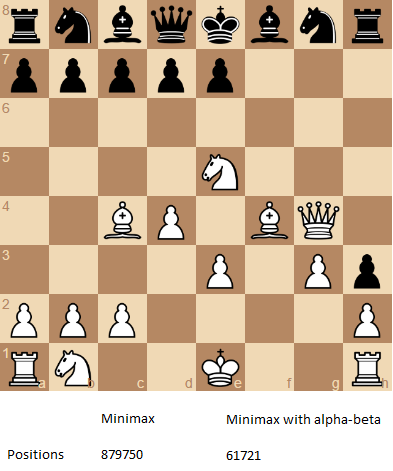
\includegraphics[width=\textwidth/2]{images/alpha-beta-example.png}

\caption{Beispielhafte Schachpositionierung \cite{Hartikka}}\label{fig:chess_example}
\end{figure}
%a step by step guide

Zur Umsetzung eines solchen Algorithmuses werden zwei Werte benötigt - $\alpha$ und $\beta$:

$\alpha$ gleicht dabei dem bisher besten (sprich höchsten) Wert in dem $\max$ Pfad des Minimax-Baums.\\
$\beta$ gleicht dagegen dem bisher besten (sprich niedrigsten) Wert in dem $\min$ Pfad des Minimax-Baums. \cite{Russell2010}

Diese Werte werden kontinuierlich aktualisiert und sobald bekannt ist, dass der Wert eines Knoten schlechter als das aktuelle $\alpha$ (bei $\max$ Ebenen) beziehungsweise $\beta$ (bei $\min$ Ebenen) sein wird, werden die restlichen Zweige dieses Knoten nicht mehr in Betracht gezogen und somit übersprungen. \cite{Russell2010}

Dies kann in einen Algorithmus verpackt werden, wie in Algorithmus \ref{alg:alpha_beta} zu sehen.

Dieser Algorithmus gleicht im Grunde dem Minimax Algorithmus, vorgestellt in Kapitel \ref{minimax} Jedoch unterscheiden die beiden Algorithmen sich um die ergänzten Werte $\alpha$ und $\beta$. Diese werden dabei jeweils in die Funktionen maxValue bzw. minValue mitgegeben. Innerhalb dieser wird dann beim Iterieren über alle erreichbaren Zustände geprüft, ob einer dieser Zustände bereits größer als $\beta$, das bisherige Minimum im min Pfad, im Fall der maxValue Funktion beziehungsweise kleiner als $\alpha$, das bisherige Maximum im max-Pfad, im Fall der minValue Funktion ist. In dem Fall wird direkt der errechnete Wert zurückgegeben und Evaluierungen aller weiteren Zustände ausgelassen, da diese ohnehin irrelevant wären.

Die Effektivität dieses Algorithmus hängt jedoch von der Reihenfolge der Evaluierung der einzelnen Zustände ab. Im besten Fall werden stets zuerst die scheinbar besten Zustände evaluiert, die ein weiteres Evaluieren der restlichen Zustände weitestgehend überflüssig machen. Im besten Fall könnte so die in Kapitel \ref{minimax} angesprochene Zeitkomplexität eines Spiels mit einer Tiefe m und einer Anzahl b an möglichen Zügen von $O(b^m)$ auf $O(b^\frac{m}{2})$ reduziert werden. Bei einer zufälligen Auswahl der Reihenfolge von zu evaluierenden Zügen dagegen würde sich die Zeitkomplexität immerhin noch auf $O(b^\frac{3m}{4})$ reduzieren. \cite{Russell2010}

Verschiedene Ansätze können dabei helfen die Reihenfolge der zu evaluierenden Züge zu verbessern. Einer dieser Ansätze ist die Züge zu sortieren, so dass zunächst die Züge evaluiert werden, bei der Figuren geschlagen werden können und daraufhin die, bei denen Bedrohungen aufgebaut werden können. Von den übrig gebliebenen Zügen werden dann zunächst die Vorwärtsbewegungen evaluiert und erst zum Schluss die Rückwärtsbewegungen. Nach diesem Schema kann die Zeitkomplexität ungefähr auf $2 \cdot O(b^\frac{m}{2})$ gebracht werden. \cite{Russell2010}

Andere Methoden sind die Züge zusätzlich danach zu sortieren, welche Züge bei vergangenen Spielen zu Erfolg geführt haben. Eine Methode dazu ist, zunächst die Züge der ersten Ebene zuerst zu evaluieren und dann eine Ebene tiefer zu gehen, die Züge dabei aber nach den Ergebnissen aus der ersten Evaluierungsiteration zu sortieren. Dies nennt sich ``Iterative Deepening''. \cite{Russell2010}

Diese Optimierung des Minimax Algorithmus spart bereits einige zu evaluierende Zustände und somit einiges an Rechenkapazitäten. Die Anzahl aller möglichen Spielzüge in Schach bleibt jedoch zu hoch, um über jeden einzelnen in angemessener Zeit zu iterieren. Auf Grund dessen muss die Tiefe, nach der die Züge evaluiert werden, reduziert werden. Ansätze dazu werden in Kapitel \ref{depth_limit} beschrieben.

\section{Problematik komplexerer Spiele}\label{depth_limit}

Der in Kapitel \ref{minimax} beschriebene Minimax-Algorithmus hat - auch mit der Optimierung durch Alpha-Beta-Pruning (Kapitel \ref{alpha_beta}) - das Problem, dass zur Entscheidungsfindung alle Pfade bis zum Ende des Spiels abgegangen werden müssen. Beim Spiel Schach beispielsweise gibt es schon nach 40 Spielzügen $10^{120}$ Möglichkeiten das Spiel zu führen. Selbst unter der sehr optimistischen Annahme, dass eine Million verschiedene Züge pro Sekunde evaluiert werden könnten, würde die Evaluation aller Spielzüge $10^{108}$ Jahre benötigen. \cite{Bernstein1958} Zum Vergleich - das Alter der Erde wird auf nicht viel mehr als $10^{9}$ Jahre geschätzt. \cite{Braterman} An dieser Tatsache ändert auch eine Reduzierung der zu evaluierenden Möglichkeiten durch Alpha-Beta Pruning nichts Wahrnehmbares.

%https://d1yx3ys82bpsa0.cloudfront.net/chess/computer-v-chessplayer.bernstein-roberts.scientific-american.june-1958.062303059.pdf
%Braterman, Paul S. (2013). "How Science Figured Out the Age of Earth". Scientific American.

Die Lösung dieses Problems scheint auf der Hand zu liegen - die Reduzierung der zu evaluierenden Züge, indem die einzelnen Pfade nicht bis zum Ende des Spiels abgegangen werden, sondern nur bis zu einer bestimmten Tiefe.

Das erste Problem bei diesem Ansatz jedoch ist, dass Spiele nicht mehr nach dem Kriterium ``Sieg'', ``Niederlage'' und ``Unentschieden'' bewertet werden können, da dies zu dem gegebenen Zeitpunkt unter Umständen noch nicht absehbar ist. Deshalb sind bei dieser Methode andere Funktionen zur Evaluierung der einzelnen Zustände nötig. Die verschiedenen Möglichkeiten zur Evaluierung der Zustände des Schachspiels werden in Kapitel \ref{evaluation} näher beschrieben.

Zum Abbrechen der redundanten Aufrufe der Funktionen bei einer gewissen Bedingung, beispielsweise einer festgelegten Tiefe, muss diese in die Abbruchbedingung der rekursiven Funktion(en) hinzugefügt werden. 

Im simpelsten Ansatz einer festgelegten Tiefe, die die einzelnen Pfade maximal durchlaufen werden, kann dies mittels einer Funktion $\mathtt{cutoff_test}$ gemacht werden, die die Parameter des aktuellen Spielzustands sowie die Tiefe übermittelt bekommt. Sie gibt den Wert wahr zurück, wenn der mitgegebene Zustand ein Endzustand oder wenn die Tiefe größer oder gleich der festgelegten Tiefe ist. \cite{Russell2010}

Wichtig ist dabei, dass bei jedem rekursiven Aufruf der Funktion der festgelegte Tiefen-Parameter stets um eins steigt, damit dieser Wert für die Abbruchfunktion zuverlässig verwendet werden kann. Als Beispiel ist hier eine modifizierte Version der maxValue Funktion aus Algorithmus \ref{alg:alpha_beta} zu sehen.

\begin{algorithm}[h]
\caption{Tiefenlimit Alpha Beta Pruning \cite{Russell2010}}
\label{alg:depth_limit}
\begin{algorithmic}
\Function{$max\_value$}{$state, \alpha, \beta, depth$}
\If{$cutoff\_test(state, depth)$} \State \Return $utility(state)$ \EndIf
\State $v \gets -\infty$
\ForAll{$a \in actions(state)$}
\State $v \gets max(v, \Call{$min\_value$}{result\_state(state, a), \alpha, \beta, depth + 1})$
\If{$v \geq \beta$} \State \Return $v$ \EndIf
\State $\alpha \gets max(\alpha, v)$
\EndFor
\State \Return $v$
\EndFunction
\\
\Function{$cutoff\_test$}{$state, depth$}
\If{$terminal\_test(state)$} \State \Return $True$ \EndIf
\If{$depth \geq MAX\_DEPTH$} \State \Return $True$ \EndIf
\State \Return $False$
\EndFunction 
\end{algorithmic}
\end{algorithm}

Ein weiterer Ansatz an Stelle einer festgelegten Tiefe ist, eine Zeit festzulegen, nach der die Rekursion abgebrochen wird. Dies hat den Vorteil, dass sich die Tiefe von selbst anpasst, je nachdem wie komplex das Spiel ist. Im Anfang des Spiels, wenn noch viele verschiedene Züge möglich sind, ist es in akzeptabler Zeit nicht möglich, sehr weit in die Tiefe zu schauen. Wenn jedoch gegen Ende des Spiels nur noch wenige Züge durchführbar sind, ist es von großem Vorteil, diese in höherem Detail zu begutachten, um den besten Zug auswählen zu können. Bei einer fixen Tiefe müsste sich auf einen Kompromiss der Tiefe geeinigt werden, um zugleich eine akzeptable Berechnungszeit zu Anfang des Spiels und eine möglichst detaillierte Betrachtung gegen Ende zu ermöglichen.

Um diese zeitbasierte Abbruchbedingung zu ermöglichen, wird ``Iterative Deepening'' verwendet. Dabei wird die Tiefe stückweise erhöht. Zunächst werden Züge also lediglich mit einer Tiefe von 1 betrachtet. Ist danach noch Zeit übrig wird die Rekursion um eine Stufe tiefer durchgeführt. Dies wiederholt sich so lange bis das Zeitlimit abgelaufen ist. \cite{Russell2010}

%pseudo code?

Dieses stückweise Vertiefen hilft zusätzlich dabei die zu betrachtenden Züge zu sortieren, um das Alpha-Beta-Pruning zu optimieren, wie in Kapitel \ref{alpha_beta} beschrieben.
Eine Gefahr bei diesen Methoden, die das Spiel nicht ganz betrachten, ist, dass die Evaluierungsfunktionen meist nur Aufschluss über den aktuellen Zustand geben, aber nicht potentielle Gefahren für die Zukunft betrachten. Gewinnt ein Spieler beispielsweise mit einem Zug einen Bauern erscheint das einer simplen, heuristischen Berechnung des Zustandes zunächst als Gewinn. Stellt der Spieler dabei jedoch beispielsweise seine Dame in eine Position, in der diese geschlagen werden kann, würde er im nächsten Zug sehr wahrscheinlich eine Figur von wesentlich höherem Wert verlieren.
Eine Möglichkeit dabei ist nur ruhende Zustände zu betrachten. Diese Methode nennt sich ``quiescence search''. Dabei werden alle Züge des zu betrachtenden Zustands, die ein Schlagen einer Figur zur Folge haben, durchgespielt. Ist keine Figur mehr zu schlagen, sondern lediglich noch Bewegungszüge möglich, so wird der Zustand als ruhig bewertet und dieser mittels der entsprechenden Funktionen evaluiert. \cite{Russell2010} \label{quiescence}

%pseudo code?

Eine andere Möglichkeit ist, die Evaluierungsfunktion dahingehend anzupassen, dass nicht nur der nächste Zustand heuristisch berechnet wird, sondern beispielsweise auch attackierte Figuren oder Schwachstellen in der Verteidigung in die Evaluation mit einzubeziehen. Darauf und generell auf möglich Evaluierungsfunktionen wird näher in dem hier folgenden Kapitel \ref{evaluation} eingegangen.
%schluss?

\section{Evaluierungsfunktionen}\label{evaluation_func}

Entscheidend für eine Schach-spielende-KI ist - neben der Anzahl der zu betrachtenden Spielzüge - die Art der Evaluation, die Aufschluss darüber geben soll, wie aussichtsreich eine bestimmte Position ist. In diesem Kapitel werden verschiedene Ansätze aufgeführt und erklärt. Dabei wird zunächst auf die Spieleröffnung eingegangen, der eine Sonderrolle im Schachspiel zukommt. Danach erfolgen die beispielhafte Nennung verschiedener Evaluierungsfunktionen im Mittelspiel ehe zum Schluss auf Strategien für das Endspiel eingegangen wird.

\subsection{Eröffnungsstrategie}\label{opening_evaluation}
Wie bereits in den einführenden Abschnitten des zweiten Kapitels erläutert, gibt es viele verschiedene Züge um ein Schachspiel durchzuführen. Damit der Spieler mit einer möglichst guten Ausgangssituation in das Spiel startet, sollten besonders die ersten Züge mit Bedacht gewählt werden. Hierbei ist es zielführend, wenn der Spieler seine Figuren direkt zu den vielversprechendsten Feldern zieht und somit in möglichst wenigen Iterationen zur gewollten Ausgangssituation kommt.\cite{O.V.}

% https://www.chesscentral.com/pages/learn-chess-play-better/chess-strategy-for-chess-openings-and-chess-principles.html

Ein Beispiel für eine gute Ausgangssituation ist es, die vier zentralen Felder d4, e4, d5, e5 zu kontrollieren. Diese Felder haben die Eigenschaft, dass ihre Lage jeder Schachfigur die jeweils größtmögliche Reichweite ermöglicht. Somit ist dies für jede Figur mitunter die gefährlichste Position im Spiel. Zum Beispiel kontrolliert ein Springer auf dem Feld d5 acht Felder, wohingegen ein Springer auf dem Feld a1 oder h1 nur zwei Felder kontrolliert (siehe Abbildung \ref{fig:knight_reach}). Ein solches explizites Vorgehen bei der Eröffnung eines Spiels nach einer speziellen Strategie, wird als Eröffnungsstragie bezeichnet.\cite{O.V.2017}

\begin{figure}[h]
\centering
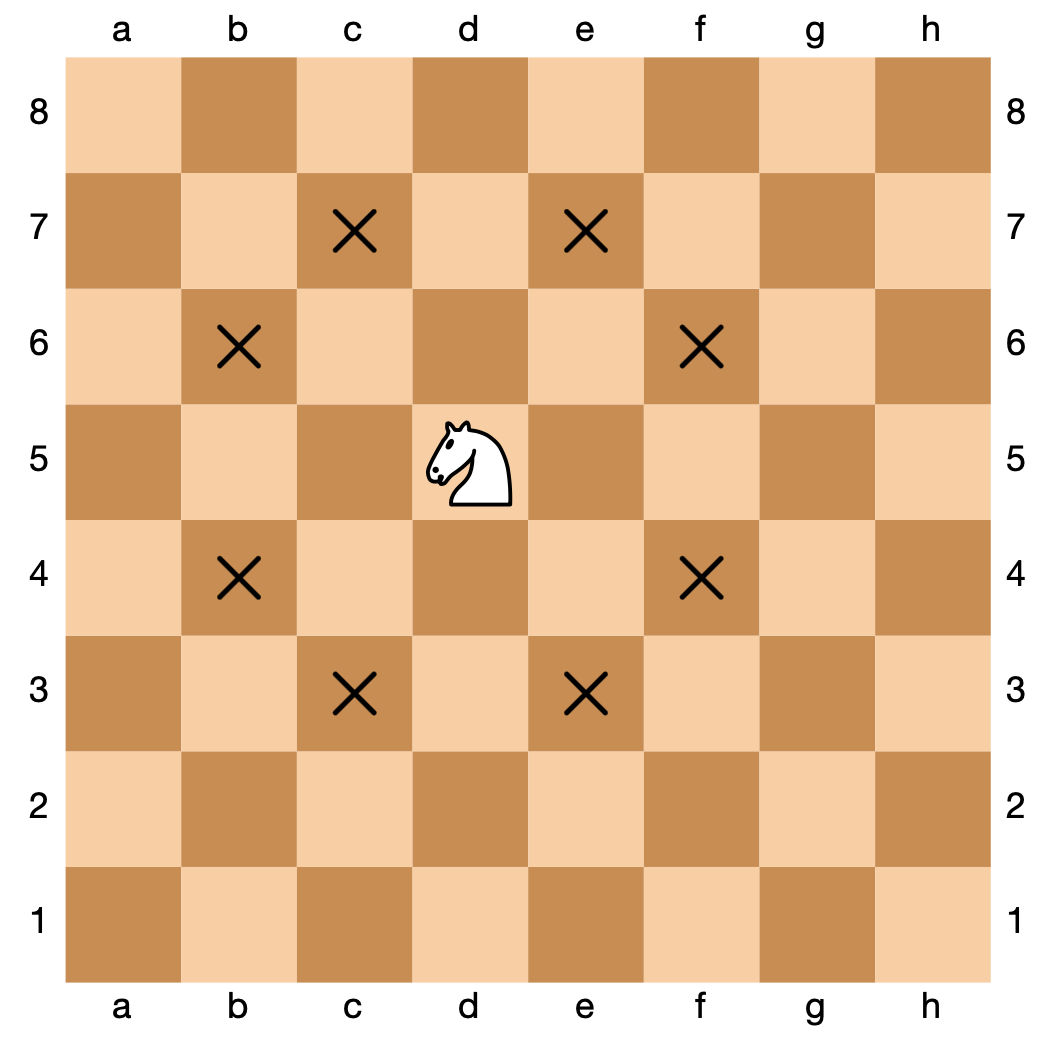
\includegraphics[width=\textwidth/2]{images/opening-books-strong-center-example.png}

\caption{Beispielhafte Reichweite eines Springers auf dem Feld d5}\label{fig:knight_reach}
\end{figure}

Durch die Verfügbarkeit von Minimax-, oder der Alpha-Beta-Suche, stellt sich die Frage, ob solche im Vorhinein festgelegten Eröffnungsstrategien nicht überflüssig sind und durch die Suche des optimalen Zugs, unter der Beachtung der vermeintlichen nächsten n-Züge, das beste Ergebnis zu Stande kommt.

Wie bereits Stuart Russell und Peter Norvig in Artificial Intelligence – A Modern Approach beschreiben, ist das Verwenden von solchen Algorithmen während der Eröffnung eines Schachspiels zu überdimensioniert und gleicht dem metaphorischen „Mit Kanonen auf Spatzen schießen“. Denn die Suche eines passenden Eröffnungszuges aus einer Anzahl von etwa einer Milliarden Spielständen ist sehr zeitaufwendig und überflüssig, wenn bspw. dies der erste Zug des kompletten Spiels ist.\cite{Russell2010} Ebenfalls ist die Wahrscheinlichkeit, dass die Eröffnungszüge eines Spiels bereits bekannt und dokumentiert sind höher, als im späteren Spielverlauf, in dem sehr viele verschiedene mögliche Züge zur Auswahl stehen.

% Hier Quelle zu Kapitel 5.4.4 Search versus lookup

Die Lösung zur Implementierung eines Eröffnungsspiels, ohne die Verwendung von komplexen Suchverfahren, liegt in den sogenannten Opening-Books. Opening-Books sind eine Ansammlung von verschiedenen dokumentierten Eröffnungsstrategien, die es ermöglichen auf eine aktuelle Spielsituation, in der Eröffnung, den passenden Zug zu finden.

Der Vorteil von Opening-Books im Gegensatz zu Suchverfahren ist, dass sie nur eine bestimmte Tiefe von Zügen unterstützen und somit deutlich schneller sind. Der deutliche Performanceunterschied erfolgt aus der Tatsache, dass in Opening-Books die besten Züge nachgeschlagen und nicht berechnet werden müssen. Ebenfalls bilden die Opening-Books sinnvolle Strategien ab, die teilweise bereits seit mehreren Jahrhunderten analysiert und verbessert wurden. Beispielsweise gibt es die Strategie ``Ruy Lopez``, oder auch die ``Spanische Eröffnung`` genannt, die bereits 1561 im Zuge der veröffentlicht des Buchs ``Libro de la invención liberal y arte del juego del ajedrez`` von Ruy López de Segura publiziert wurde. Somit müssen nicht erst Berechnungen durchgeführt werden, die bemessen, ob bzw. inwiefern ein Zug in dieser Situation zielführend ist oder nicht. Stattdessen wird auf eine Datenbank von Zügen und deren Bemessungen zurückgegriffen.\cite{Chess.comTeamInternational2018}

% https://www.chess.com/article/view/the-ruy-lopez-chess-opening-explained

Sobald eine Strategie abgeschlossen ist oder das Opening-Book keinen sinnvollen Zug mehr auf eine komplexe Spielsituation hat, kommen die bereits eingeführten Suchverfahren zum Einsatz.

Der Nachteil der Opening-Books ist, dass diese nicht für jeden im Eröffnungsspiel getätigten Zug des Gegners eine passende Strategie besitzen. Die Opening-Books gehen davon aus, dass der Gegner ein Spieler ist, der auch professionelle Eröffnungsstrategien spielen wird und somit möglichst schnell die besten Felder mit seinen Figuren zu kontrollieren. Wenn es dazu kommt, dass ein Spieler durch Unwissenheit, oder bewusst nicht die vermeintlich besten Züge zur Eröffnung spielt, sondern Züge, die nicht im Opening-Book vorkommen, dann gibt es keine Strategie zu der aktuellen Spielsituation und das Opening-Book kann nicht mehr eingesetzt werden. 

Damit das Schachspiel trotz der Tatsache, dass das Opening-Book keine sinnvolle Strategie liefern kann, fortgesetzt werden kann, muss Gebrauch von Suchverfahren gemacht werden. Hierbei ist zu beachten, dass dies, im Gegensatz zu Opening-Books, negative Auswirkungen, auf die im Eröffnungsspiel benötigte Zeit zur Berechnung von Zügen hat.

% https://www.thesprucecrafts.com/most-common-chess-openings-611517 Nur versch. Strategien
% http://www.thechesswebsite.com/chess-openings/ Nur versch. Strategien

% Was sind Eröffnungsstrategien
% Warum sollte man diese nutzen
% Wieso besser als alpha beta pruning
% Was sind Opening-Books
% Wo liegen die Stärken von Opening-Books?
% Wo liegen die Schwächen von Opening-Books

\subsection{Figurenbewertung (+ Position)}\label{material_evaluation}

Der wohl simpelste und gängigste, aber auch wichtigste Ansatz zur Evaluierung eines Schachbretts ist die heuristische Bewertung der auf dem Brett vorzufindenden Materialien. Dies bedeutet, dass die Figuren beider Spieler gezählt und voneinander subtrahiert werden. Das Ergebnis dieser Rechnung gibt Aufschluss darüber, welcher Spieler sich momentan in der aussichtsreicheren Position befindet.

Da jedoch nicht alle Figuren vom gleichen Wert sind, ist es vorteilhaft den einzelnen Figuren einen Faktor zuzuweisen, der Aufschluss über diesen gibt. Dies nähert die Funktion der Wertschätzung des Schachbretts an den tatsächlichen Wert an, da zwei Türme beispielsweise wichtiger als zwei Bauern sind. Im Ansatz ohne Faktorisierung der verschiedenen Spielfiguren würde dies keine Beachtung finden.

Claude Shannon hat dazu 1949 den einzelnen Figuren folgende Werte zugewiesen, die seitdem als Richtwerte für Evaluierungen gelten. \cite{Shannon1950}

\begin{tabular}{ l c r }
\textbf{Bauer} & 1\\
\textbf{Springer} & 3 \\
\textbf{Läufer} & 3 \\
\textbf{Turm} & 5 \\
\textbf{Dame} & 9 \\
\textbf{König} & 200
\end{tabular}

%https://www.pi.infn.it/~carosi/chess/shannon.txt

Die Berechnung des Wertes eines Schachbretts kann dann wie folgt aussehen:

\begin{equation}
\begin{aligned}
f() = 200 \cdot (K_w-K_b) + 9 \cdot (Q_w-Q_b) + 5 \cdot (R_w-R_b) + \\3 \cdot (B_w-B_b) + 3 \cdot (N_w-N_b) + 1 \cdot (P_w-P_b) \cite{Shannon1950}
\end{aligned}
\end{equation}

%https://www.pi.infn.it/~carosi/chess/shannon.txt

wobei K für König steht, Q für Dame, R für Turm, B für Läufer, N für Springer und P für Bauer. Die untergestellten Zeichen w und b stehen für weiß und schwarz.

Diese Berechnung gibt bereits einen recht guten Aufschluss über den Wert des Spiels. Noch besser wird diese heuristische Berechnung jedoch, wenn dabei auch die Positionen dieser Figuren mit einbezogen werden. Dazu hat Tomasz Michniewski folgende Matrizen vorgeschlagen \cite{O.V.2019a}

\begin{table}[htbp]
\tiny
\newcolumntype{P}{>{\centering\arraybackslash}p}
\begin{tabular}{@{}P{\textwidth/100*47} P{\textwidth/100*47}}
\textbf{Bauer} & \textbf{Springer}\\
\begin{tabular}{@{}c c c c c c c c}
0&0&0&0&0&0&0&0\\
50&50&50&50&50&50&50&50\\
10&10&20&30&30&20&10&10\\
5&5&10&25&25&10&5&5\\
0&0&0&20&20&0&0&0\\
5&-5&-10&0&0&-10&-5&5\\
5&10&10&-20&-20&10&10&5\\
0&0&0&0&0&0&0&0
\end{tabular}
&
\begin{tabular}{c c c c c c c c}
-50&-40&-30&-30&-30&-30&-40&-50\\
-40&-20&0&0&0&0&-20&-40\\
-30&0&10&15&15&10&0&-30\\
-30&5&15&20&20&15&5&-30\\
-30&0&15&20&20&15&0&-30\\
-30&5&10&15&15&10&5&-30\\
-40&-20&0&5&5&0&-20&-40\\
-50&-40&-30&-30&-30&-30&-40&-50\\
\end{tabular}
\end{tabular}\\
\begin{tabular}{@{}P{\textwidth/100*47} P{\textwidth/100*47}}
\textbf{Läufer} & \textbf{König}\\
\begin{tabular}{@{}c c c c c c c c}
-20&-10&-10&-10&-10&-10&-10&-20\\
-10&0&0&0&0&0&0&-10\\
-10&0&5&10&10&5&0&-10\\
-10&5&5&10&10&5&5&-10\\
-10&0&10&10&10&10&0&-10\\
-10&10&10&10&10&10&10&-10\\
-10&5&0&0&0&0&5&-10\\
-20&-10&-10&-10&-10&-10&-10&-20
\end{tabular}
&
\begin{tabular}{c c c c c c c c}
-30&-40&-40&-50&-50&-40&-40&-30\\
-30&-40&-40&-50&-50&-40&-40&-30\\
-30&-40&-40&-50&-50&-40&-40&-30\\
-30&-40&-40&-50&-50&-40&-40&-30\\
-20&-30&-30&-40&-40&-30&-30&-20\\
-10&-20&-20&-20&-20&-20&-20&-10\\
20&20&0&0&0&0&20&20\\
20&30&10&0&0&10&30&20
\end{tabular}
\end{tabular}\\
\begin{tabular}{@{}P{\textwidth/100*47} P{\textwidth/100*47}}
\textbf{Dame} & \textbf{Turm}\\
\begin{tabular}{@{}c c c c c c c c}
-20&-10&-10&-5&-5&-10&-10&-20\\
-10&0&0&0&0&0&0&-10\\
-10&0&5&5&5&5&0&-10\\
-5&0&5&5&5&5&0&-5\\
0&0&5&5&5&5&0&-5\\
-10&5&5&5&5&5&0&-10\\
-10&0&5&0&0&0&0&-10\\
-20&-10&-10&-5&-5&-10&-10&-20
\end{tabular}
&
\begin{tabular}{c c c c c c c c}
0&0&0&0&0&0&0&0\\
5&10&10&10&10&10&10&5\\
-5&0&0&0&0&0&0&-5\\
-5&0&0&0&0&0&0&-5\\
-5&0&0&0&0&0&0&-5\\
-5&0&0&0&0&0&0&-5\\
-5&0&0&0&0&0&0&-5\\
0&0&0&5&5&0&0&0
\end{tabular}
\end{tabular}
\end{table}

Diese Matrizen können ergänzend zur Berechnung des Spielwertes genommen werden, um die Positionen der einzelnen Schachfiguren mit einbeziehen zu können. Dazu wird für alle Figuren der Wert aus der entsprechenden Position genommen, diese Werte zusammenaddiert und durch 100 geteilt.

Mittels Kombination aus diesen heuristischen Messmethoden kann bereits eine aufschlussreiche Zahl berechnet werden, wie aussichtsreich das aktuelle Spiel für den jeweiligen Spieler ist. Verstärkt werden kann dies jedoch durch weitere Funktionen, die auch Angriff, Verteidigung und Beweglichkeit des Spiels mit einbeziehen.

%https://www.chessprogramming.org/Simplified_Evaluation_Function

\subsection{Verteidigung}\label{defense_evaluation}

Um die Stärke der Verteidigung eines Spielers zu messen, gilt vor Allem die Verteidigung des Königs als Messwert dafür. Dabei gibt es verschiedene Strategien.

Eine dabei ist die Position der Bauern zu messen, um herauszufinden, inwiefern das sogenannte ``Bauern Schild'' intakt ist. Ein Bauern Schild existiert dann, wenn der König durch vorstehende Bauern geschützt ist und keine Figur den König bedrohen kann, ohne vorher an diesem vorbei zu kommen. Eine Lücke in einem solchen Schild sollte dabei zu einer negativen Bewertung des Spielzustands führen. Dies kann noch dahingehend erweitert werden, dass eine Lücke in dem Bauern Schild umso höher in die Bewertung mit einfließt, desto mehr Material, also Figuren multipliziert mit ihren Werten, der Gegner noch auf dem Schachbrett hat. Dies führt dazu, dass die KI in dem Fall einer Lücke eher zu einem Figurentausch neigt, um Gefahren für den König zu eliminieren, wenn es an seiner eigenen Verteidigung mangelt. \cite{O.V.2019b}

Ein weiterer Ansatz ist den Angriff auf die Königs-Zone zu messen und entsprechend zu bewerten. Die Königszone wird dabei definiert auf die um den König umliegenden Felder plus zwei bis drei weitere Felder voraus in Richtung des Gegenspielers. In Abbildung \ref{fig:king_zone} werden diese Felder rot markiert.

\begin{figure}[h]
\centering
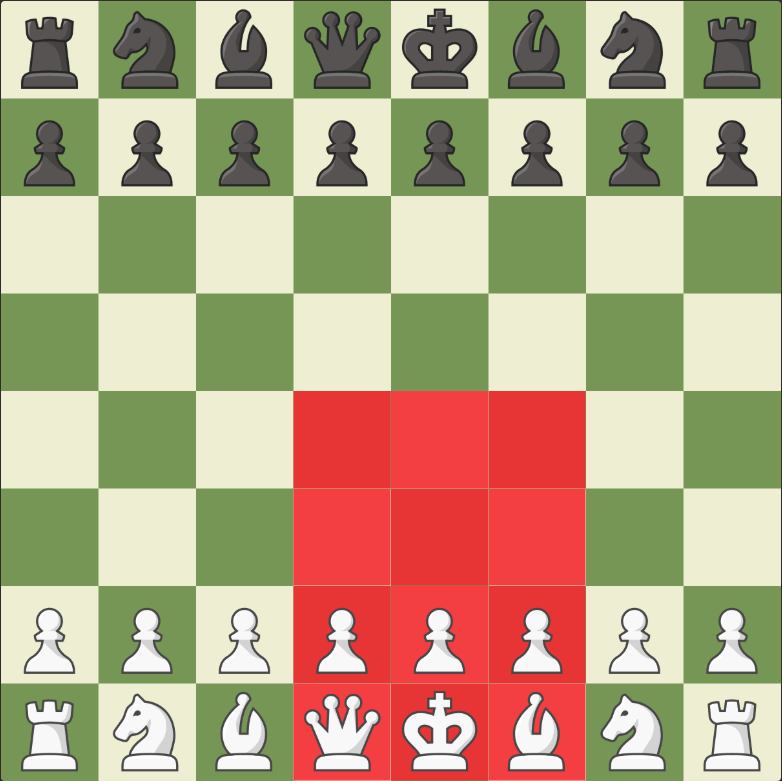
\includegraphics[width=\textwidth/5*3]{images/king_zone.PNG}

\caption{Königszone im Schachspiel vom Ausgangszustand \cite{}}\label{fig:king_zone}
\end{figure}

Dann wird die Zahl der Figuren des Gegners gemessen, die diese Felder angreifen können. Dies wird in einer Variable ``attacking\_pieces\_counter'' gespeichert. Anhand dieser Zahl wird das Gewicht ``attack\_weight'' bestimmt. Dies kann folgender Tabelle entnommen werden: \cite{O.V.2019b}

\begin{tabular}{c c}
\textbf{attacking\_pieces\_counter} & \textbf{attack\_weight}\\
1 & 0\\
2 & 50\\
3 & 75\\
4 & 88\\
5 & 94\\
6 & 97\\
7 & 99
\end{tabular}

Zusätzlich wird der Wert der Angriffe berechnet. Dazu wird für jede Figur, die die König-Zone angreifen kann, gezählt, wie viele Felder innerhalb dieser die Figur erreichen kann. Dies wird dann mit einer Konstante multipliziert abhängig vom Typ der Figur - 20 für einen Springer, 20 für einen Läufer, 40 für einen Turm und 80 für eine Dame. Für jede angreifende Figur wird diese Berechnung durchgeführt und das Ergebnis zur Variable ``value\_of\_attacks'' hinzugefügt.  \cite{O.V.2019b}

Abschließend werden diese berechneten Werte ``attack\_weight'' und ``value\_of\_attacks'' miteinander multipliziert und das Ergebnis durch 100 dividiert, wie in folgender Gleichung zu sehen: \cite{O.V.2019b}

\begin{equation}
(value\_of\_attacks  \cdot  attack\_weight[attacking\_pieces\_counter]) / 100)
\end{equation}

Dieser Wert gibt dann guten Aufschluss darüber, wie gut oder schlecht die Sicherheit des Königs gewährleistet wird. Dabei werden jedoch nur Offiziersfiguren betrachtet.

Mittels dieser Ansatzes ist es möglich die Sicherheit seines eigenen Königs zu berechnen. Dies ist ein besonders wichtiger Ansatz bei der Evaluation eines Spielzustandes, damit die KI den eigenen König nicht unbedacht offen stellt, was langfristige, negative Folgen für sein Spiel haben kann. 

%https://www.chessprogramming.org/King_Safety

\subsection{Angriff}\label{offense_evaluation}

Neben der Verteidigung spielen auch die Möglichkeiten zum Angriff auf den Gegner eine Rolle, um einen Spielzustand zu evaluieren.

Ein erster, simpler Ansatz ist dabei neben dem Wert der Materialien auch die möglichen Angriffe auf Figuren mit in die Evaluation mit einzubeziehen. Auch dabei gilt es den Wert der angegriffenen Funktion mit einzuberechnen sowie die Anzahl der angreifenden Figuren. Am Ende müssen diese Werte sowohl für von schwarz angegriffene als auch von weiß angegriffene Figuren berechnet und voneinander subtrahiert werden, um den Vorteil im Angriff berechnen zu können. Diese Möglichkeit der Evaluation ist nur dann möglich, wenn es sich nicht um einen ruhigen Zustand handelt, wie in Kapitel \ref{quiescence} erklärt. 

Ein weiterer, wichtiger Ansatzpunkt für aufbauende Angriffe ist die Kontrolle des Zentrums. Beim Zentrum handelt es sich dabei um die Felder d4, d5, e4 und e5. Dies ist ein wichtiger Ansatz bei in Kapitel \ref{opening_evaluation} beschriebenen ``Opening-books'', sowie bei in Kapitel \ref{material_evaluation} beschriebenen Matrizen zur Bewertung der Positionierung der Figuren auf einem Schachbrett. 

Um dies dennoch extra zu evaluieren, kann durch alle Figuren durchiteriert werden. Dabei wird nach den Figuren gefiltert, denen es möglich ist im nächsten Zug das Zentrum des Spielfeldes zu erreichen. Anschließend werden diese Figuren mit ihren zugehörigen Werten multipliziert und die Ergebnisse daraus aufsummiert. Letzlich wird dies für beide Farben durchgeführt und die Differenz zwischen der Werte der verschiedenen Farben zurück gegeben. \cite{O.V.2019}

%https://www.chessprogramming.org/Center_Control

Um Angriffe effizient aufbauen zu können, ist auch Mobilität ein wichtiger Faktor im Spiel. In einer Studie von Eliot Slater wurde deutlich, dass die Anzahl der durchführbaren Züge bei gleichzeitiger Gleichheit der verfügbaren Materialien eine deutliche Korrelation mit der Anzahl der gewonnenen Spiele zeigt. \cite{Slater1988}

Der simpelste Ansatz, um diese messbar zu machen, ist schlicht den benannten Wert der Anzahl der Züge zur Hilfe zu nehmen und diese für beide Spieler zu vergleichen.

Dies kann jedoch noch um verschiedene Faktoren erweitert werden. Dies ist beispielsweise Vorwärtsbewegungen höher zu bewerten als Rückwärtsbewegungen oder vertikale Bewegungen höher als horizontale. Ebenso können auch Züge mitgezählt werden, die auf ein Feld führen, das bereits von einer befreundeten Figur belegt ist. Dies stellt zwar keinen legalen Zug dar, sichert jedoch die befreundete Figur ab. \cite{O.V:2019}

%https://www.chessprogramming.org/Mobility

Zudem kann zur Bewertung eines Angriffs auch die Sicherheit des gegnerischen Königs zur Hilfe genommen werden. Wie diese berechnet wird, ist in Kapitel \ref{defense_evaluation} aufgeführt.

All diese Kriterien führen zu einer guten Möglichkeit Angriffe beziehungsweise den Aufbau von Angriffen bewerten zu können und gehen somit über die beschriebene Defensivstrategie hinaus.

%Blockierte Bauern?
%Trap?

\subsection{Spielverlauf}\label{history_evaluation}

Neben den bisher beschriebenen heuristischen Funktionen zur Bewertung eines Spiels, kann auch statistische Bewertung Einfluss auf diese nehmen.

Dazu ist es wichtig, eine möglichst große Historie an Spielen aufzubauen. Dazu kann im Laufe eines Spiels jeder einzelne Zustand abgespeichert werden, so dass dieser eindeutig identifizierbar ist. Am Ende des Spiels muss dazu dann ein Wert hinzugefügt werden, der Aufschluss über Sieg, Unentschieden oder Niederlag gibt. Dazu können die Werte 1, 0 und -1 dienen.

Beim Zusammenfügen der Historie des aktuellen Spiels mit der aufzubauenden Gesamthistorie aller Spiele gilt es dann über die Historien zu iterieren und nach gleichen Zuständen zu suchen. Diese gilt es dann zu migrieren, um eine Statistik aufzubauen, die Aufschluss über die Anzahl aller Siege und Niederlagen ausgehend von dem speziellen Zustand zu gewinnen.

Die Aussagekraft ist vor Allem dann kräftig, umso höher die Zahl ist. Wenn es sich um lediglich eine positive Bilanz von ein oder zwei Siegen mehr als Niederlagen handelt, kann dies schlicht an der geringen Zahl an Vorkommnissen des Zustands liegen. Ist dieser jedoch sehr hoch, ist ein Zufall eher unwahrscheinlich.

Deshalb gilt es eine möglichst große Historie aufzubauen, die vor Allem in der Anfangsphase, in der noch nicht so viele verschiedene Zustände erreichbar sind, guten Aufschluss über die Qualität des Zustands geben kann. Umso fortgeschrittener jedoch das Spiel ist, desto schwieriger wird es eine angemessene Anzahl an Iterationen über die speziellen Zustände zu erreichen, da diese immer häufiger vorkommen.

Da im Spiel Schach $10^{40}$ verschiedene Spielzustände existieren \cite{Stroetmann2018} , ist es kaum möglich alle Zustände in angemessener Anzahl durchgegangen zu sein und abzuspeichern. Selbst unter der Annahme, dass ein Zustand inklusive dessen Bilanz in nur 20 Bit gespeichert werden kann (12 Bits für Schachspiel \cite{Speight} und 8 Bits für Bilanz), würde dies 

\begin{equation}
\begin{aligned}
10^{40}  \cdot  20 Bits = 2  \cdot  10^{41} Bits = 2,5  \cdot  10^{40} Bytes = 2,5  \cdot  10^{25} Petabytes
\end{aligned}
\end{equation}

an Speicherplatz benötigen, was eine unverhältnismäßige Größe darstellt. Zudem würde die Ansammlung dieser Daten unverhältnismäßig lange dauern.

%https://codegolf.stackexchange.com/questions/19397/smallest-chess-board-compression

Aus diesem Grund stellt dies zwar eine gute Größe für den Beginn des Spiels dar, verliert jedoch im späteren Spielverlauf auf Grund fehlender Vorkommnisse der Zustände an Aussagekraft.

% Computer Chess Compendium

\subsection{Endspiel}\label{finishing_evaluation}
Nach dem Eröffnungsspiel und dem Mittelteil einer Schachpartie, folgt das Endspiel. Das Endspiel beschreibt dabei eine Situation, bei der sich nur eine geringe Anzahl an schwarzen und weißen Figuren auf dem Schachbrett befinden. 

Zum zielstrebigen Gewinnen des Spiels, ohne überflüssige Züge, ist es hilfreich sich grundlegende Muster anschauen, die es ermöglichen den Gegner Schachmatt zu setzen. Neben der Möglichkeit zielstrebig und effizient das Spiel gewinnen zu können, kann das Wissen über solche Muster auch dazu beitragen den Gegner vom Gewinnen abzuhalten, da ersichtlicher wird was dessen Strategie ist.

In Abbildung \ref{fig:RKvk} findet man eine simple Endspielsituation vor, in der die Partei mit den weißen Figuren die gegnerische Partei trivial Schachmatt setzen kann, da die schwarze Partei nur noch den König als Figur besitzt und sich einem Turm und einem König gegenüber sieht.

\begin{figure}[h]
\centering
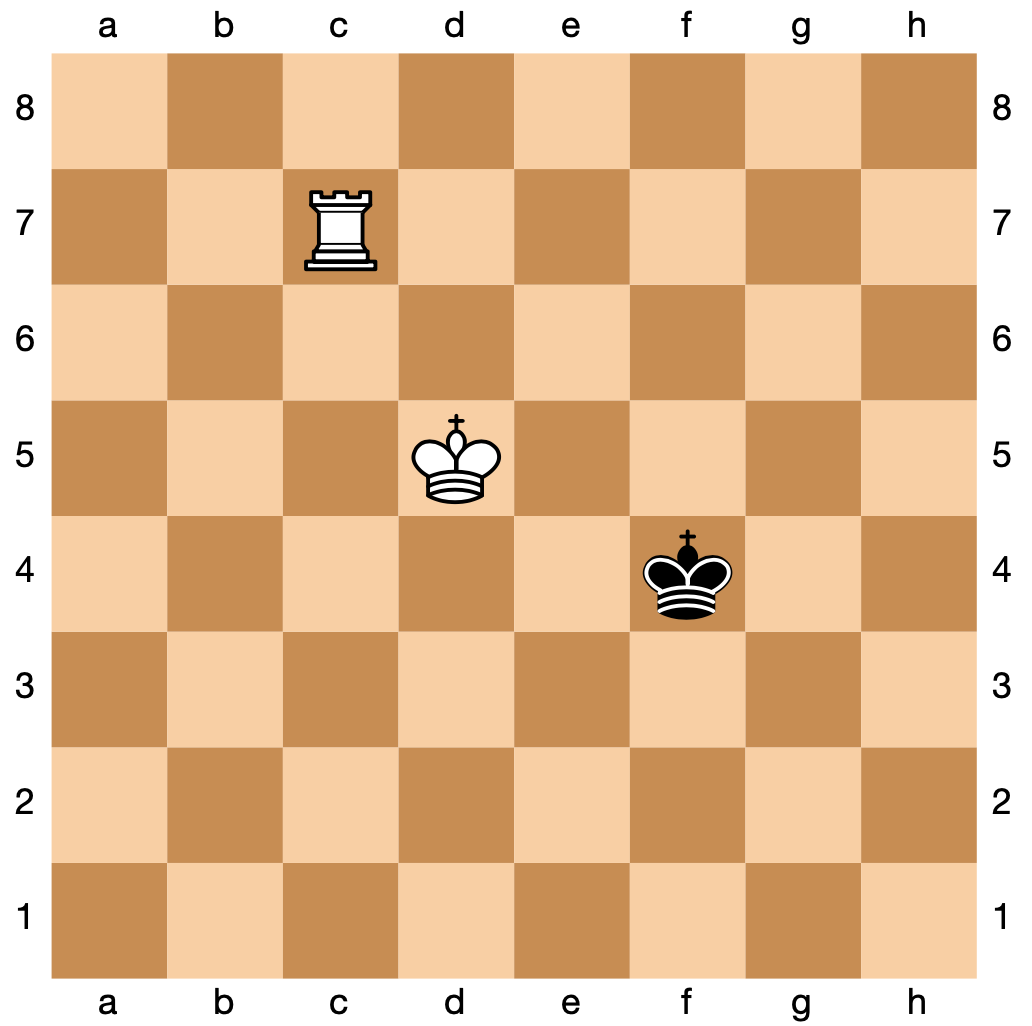
\includegraphics[width=\textwidth/5*4]{images/RKvk.png}

\caption{Endspielsituation RKvk}\label{fig:RKvk}
\end{figure}

Ein Ausweg aus der drohenden Niederlage ist die 50-Züge-Regel, mittels der die schwarze Partei ein Remis erzielen kann. Für die Erfüllung dieser Regel muss nachgewiesen werden, dass in den letzten 50 Zügen keine Figur geschlagen oder ein Bauer gezogen wurde.\cite{Alt2018} Um das Spiel zu gewinnen muss somit die weiße Partei zielstrebig den schwarzen König Schachmatt setzen.

% Quelle Regel: FIDE-Regeln-2018-Final-DEU.pdf https://www.schachbund.de/satzung-ordnungen.html?file=files/dsb/srk/downloads/FIDE-Regeln-2017-Final-DEU-ENG.PDF

Im Laufe der Jahre seitdem es das Schachspiel gibt wurden bereits einige Endspiele analysiert und evaluiert um daraus mögliche Muster und Strategien zu erhalten, die zu einem Sieg in einem Endspiel führen können. Diese vorliegenden Analysen helfen bei der Umsetzung einer Schach-KI, da mittels solcher Informationen schnell evaluiert werden kann welcher Zug am Gewinnbringendsten für den Spieler ist. 

Theoretisch lässt sich auch durch die Verwendung von Suchalgorithmen, wie das bereits vorgestellte Alpha-Beta-Pruning, der beste Zug ermitteln, jedoch kann dies deutlich länger dauern als das Zurückgreifen auf bereits durchgeführte Analysen. Dies hat den Grund, da beispielsweise bereits bei drei verschiedenen Figuren, die sich zu Ende des Spiels auf dem Brett befinden, eine sehr große Anzahl an verschiedenen Zugmöglichkeiten ergibt. Dies ist unter anderem darin begründet, dass diese drei verbliebenen Figuren aus einer unterschiedlichen Konstellation aus Steinen bestehen. Neben den beiden Königen kann der dritte Stein jeder beliebige andere als ein König sein. Dabei hat diese dritte Figur pro Stein unterschiedliche Sprungeigenschaften, wie bspw. Distanz und Richtung. Ebenfalls hat die Position, auf der sich die Figuren befinden einen großen Einfluss auf die Möglichkeiten. Somit ergibt sich in Summe für ein Endspiel mit drei Figuren bereits eine Anzahl von 368.079 (siehe \ref{table:nulp}) verschiedenen Positionen.

\begin{center}
\begin{tabular}{| p{5cm} | p{5cm} |}
\hline
\textbf{Anzahl der Figuren} & \textbf{Mögliche Positionen}\\ \hline
2 & 462\\ \hline
3 & 368.079\\ \hline
4 & 125.246.598\\ \hline
5 & 25.912.594.054\\ \hline
6 & 3.787.154.440.416\\ \hline
7 & 423.836.835.667.331\\ \hline
8 & 38.176.306.877.748.245 \cite{Kryukov2014}\\
\hline
\end{tabular}
\label{table:nulp}
\end{center}
% http://kirill-kryukov.com/chess/nulp/results.html

Zum aktuellen Zeitpunkt wurden alle möglichen Züge der letzten sieben Steine auf einem Schachbrett berechnet und liefert somit der zu programmierenden KI eine Datenbank mit vielen verschiedenen Zügen und den jeweils besten davon.


% Was ist das Endgame?
% Einer versucht zu gewinnen, der andere versucht ein Remi zu erreichen
% Was ist das besondere an dem Endgame?
% Wieso sollte man hier keine Such-Algorithmen verwenden?